\chapter{Example chapter}\label{chap:sample}

\section{Text}\label{chap:exp:sec:background}

Small Caps font: \textsc{HkustThesis}

\subsection{Cross references}

You can use \lstinline|\cref{}| to automatically setup the cross reference name; instead, you can always use \lstinline|\ref{}| to customize the appearance of the cross reference.

Chapter \ref{chap:introduction} tells you to read the latest PDF documentation.

\cref{chap:conclusions} is a conclusion.

\subsection{Citation and bibliography}

Use \lstinline|biber| as \hologo{BibTeX} backend.

Cite a book\cite{LaTeX.Companion}, some papers\cite{KeshavACMSIGCOMMComput.Commun.Rev.2007, WhitesidesAdv.Mater.2004}, and a conference\cite{, Babu2020IEEE33rdInt.Conf.MicroElectroMech.Syst.MEMS2020}.

\subsubsection{Citation database}

Bibliography entries (database) are stored in \lstinline|mythesis.bib|. You can use Zotero (or similar software) to generate \lstinline|another.bib| file. You can add multiple database files by adding their filenames one-by-one in the following commands in \lstinline|mythesis.tex|:

\begin{lstlisting}[language=TeX]
\addbibresource{mythesis.bib}
\addbibresource{another.bib}
\end{lstlisting}

\subsubsection{Citation style}

As described in the sample page from ECE department, the style is set to \lstinline|ieee| by default. You can modify the style in the \lstinline|hkustthesis.cls| file as you wish.

\section{Math}

\subsection{Symbols}

\begin{itemize}
  \item Calligraphic letters: $\mathcal{A}$
  \item Mathbb letters: $\mathbb{A}$
  \item Mathfrak letters: $\mathfrak{A}$
  \item Math Sans serif letters: $\mathsf{A}$
  \item Math bold letters: $\mathbf{A, \alpha, \Sigma}$ \, (\lstinline|\mathbf|)
  \item Math bold letters: $\symbfup{A, \alpha, \Sigma}$ \, (\lstinline|\symbfup|)
\item Math bold italic Greek letters\footnote{Avoid using \lstinline|bm| package as it conflicts with \lstinline|unicode-math| and it is outdated for \hologo{XeLaTeX}. You can alias some math commands by \lstinline|\\newcommand| or \lstinline|\\renewcommand| anyway.}: $\bm{\alpha}$
  \item Math bold italic Greek letters in upper case: $\mathbi{A}$
\end{itemize}

\subsection{Equations}

\begin{equation}
  E^2 = m^2 + p^2\label{eq:mass-energy}
\end{equation}

\cref{eq:mass-energy} or Equation (\ref{eq:mass-energy}) gives the mass-energy relationship.

\subsection{Theorem}

\begin{definition}
  LCL is orange juice.
\end{definition}

\begin{proof}
  They are both orange.
\end{proof}

\begin{algorithm}[htbp]
  \caption{Temp}
  \begin{algorithmic}[1]
    \STATE Temp
  \end{algorithmic}
\end{algorithm}

Available theorem environments are listed below:

algorithm, assumption, axiom, conclusion, condition, corollary, definition, example, lemma, proof, property, proposition, remark, theorem.

\section{Figure}
An example image is shown in \cref{fig:tikz example} or Figure (\ref{fig:tikz example}).

\begin{figure}[H]
  \centering
  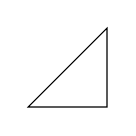
\begin{tikzpicture}
    \draw (0,0) -- (1, 0) -- (1, 1) -- cycle;
  \end{tikzpicture}
  \caption{An example tikz picture with a short caption.}
  \label{fig:tikz example short}
\end{figure}

\begin{figure}[H]
  \centering
  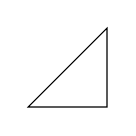
\begin{tikzpicture}
    \draw (0,0) -- (1, 0) -- (1, 1) -- cycle;
  \end{tikzpicture}
  \caption{An example tikz picture with breakline and\\ a very very very very very very very very very very very very very very very very very very very very very very very very very very very very very very very long caption.}
  \label{fig:tikz example}
\end{figure}

\section{Table}

An example table is shown in \cref{tab:environment} or Table (\ref{tab:environment}).

\begin{table}[H]
  \centering
  \caption{A table with a short caption.}
  \label{tab:table_short}
  \begin{tabular}{lll}
    \toprule
    OS           & TeX environment                & Test                                \\
    \midrule
    Overleaf     & \hologo{TeX}\,Live 2021$\sim$4 & Pass                                \\
    Windows 10   & \hologo{TeX}\,Live 2020        & \color{red}{\verb|ltxhook| problem} \\
    Ubuntu 20.04 & \hologo{TeX}\,Live 2021        & Pass                                \\
    \bottomrule
  \end{tabular}
\end{table}

\begin{table}[H]
  \centering
  \caption{Test result on different platforms with breakline and\\ a very very very very very very very very very very very very very very very very very very very very very very very very very very very very very very very long caption.}
  \label{tab:environment}
  \begin{tabular}{lll}
    \toprule
    OS                   & TeX environment                & Test                                \\
    \midrule
    Overleaf             & \hologo{TeX}\,Live 2021$\sim$4 & Pass                                \\
    Arch Linux (2024.10) & \hologo{TeX}\,Live             & Pass                                \\
    Windows 10/11        & \hologo{TeX}\,Live 2021        & Pass                                \\
    macOS 10.15          & \hologo{TeX}\,Live 2021        & Pass                                \\
    Windows 10           & \hologo{TeX}\,Live 2020        & \color{red}{\verb|ltxhook| problem} \\
    Ubuntu 20.04         & \hologo{TeX}\,Live 2021        & Pass                                \\
    Termux               & \hologo{TeX}\,Live 2021        & Pass                                \\
    Windows 11           & \hologo{MiKTeX} 4.9            & Pass                                \\
    Windows 10           & \hologo{MiKTeX} 4.4            & Pass                                \\
    \bottomrule
  \end{tabular}
\end{table}

\section{Code}

\subsection{Inline code}
Use \lstinline$\lstinline|<code>|$ to print code snippets. The \lstinline$||$ marks delimit
the code and can be replaced by any character not in the code;
\eg \lstinline|\lstinline$<code>$| gives the same result.

\subsection{Code environment}
The code to draw the \cref{fig:tikz example} is listed below:
\begin{lstlisting}[caption={\hologo{LaTeX} code for inserting a figure}]
\begin{figure}[htb]
  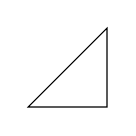
\begin{tikzpicture}
    \draw (0,0) -- (1, 0) -- (1, 1) -- cycle;
  \end{tikzpicture}
  \caption{An example picture with long caption: \blindtext\\\blindtext}
  \label{fig:tikz example} % this is a comment
\end{figure}
\end{lstlisting}
